\subsection{Di-bosons backgrounds}

WZ and ZZ production with the gauge boson decaying to electrons, muons or taus can yield the same leptonic final states as the signal, if considering also events where not all leptons are identified. While the ZZ background is greatly reduced by the cut on MET LD, the WZ background remains an important contribution to the three and more leptons signal region.

When not requiring additional hadronic jets in the final states, these processes are predicted theoretically at NLO accuracy, and the inclusive cross sections have been successfully measured at the LHC. However these good agreement does not translate automatically to the signal regions used in this search, which always require the presence of at least one b-tagged jet.

Since dibosons are preferentially produced in association with jets from light quarks or gluons, it is possible to isolate a clean control region of WZ plus hadronic jets by inverting the b-tagging requirements of the signal region and also inverting the $Z \rightarrow ll$ veto. The approach chosen for estimating the background is therefore to use simulated events but normalizing the overall event yields in control regions of WZ plus two not b-tagged jets. This reduces the systematic uncertainty on the prediction, since the theoretical uncertainty on the ratio of event yields between signal region and control region is much smaller than the uncertainty on the production cross section of diboson plus multijet. The majority of events from this background in the signal region contain jets from gluons or light quarks mistagged as b-jets, for which the extrapolation is affected only by uncertainties of experimental origin.

\subsubsection{Measurement in data from events with no b-jets}
\textcolor{red}{This part is being updated with the full 2016 data. However, the plots in the WZ$\rightarrow$3l control region in Sec. \ref{sec:WZ control region}  show already a scale factor compatible with unity between data and simulation.}

The extraction of the WZ yield in the control region is performed via a one dimensional negative log likelihood fit of the shape of transverse mass of the lepton not associated to the Z boson. The shape and normalization of the residual backgrounds are fixed to the expectations from simulations. The measurement has been performed on 35.9\fbinv data collected in 2016, and yields a scale factor of $0.96\pm 0.06\text{ (stat.)}$.

Figures ~\ref{fig:RescalingWZ} show the good agreement observed in the WZ control region for the following distributions:

\begin{itemize}
     \item $m_{T} W(l)$
     \item $E_{T}^{miss}$ 
\end{itemize}

\begin{figure}[htp]
	\centering
	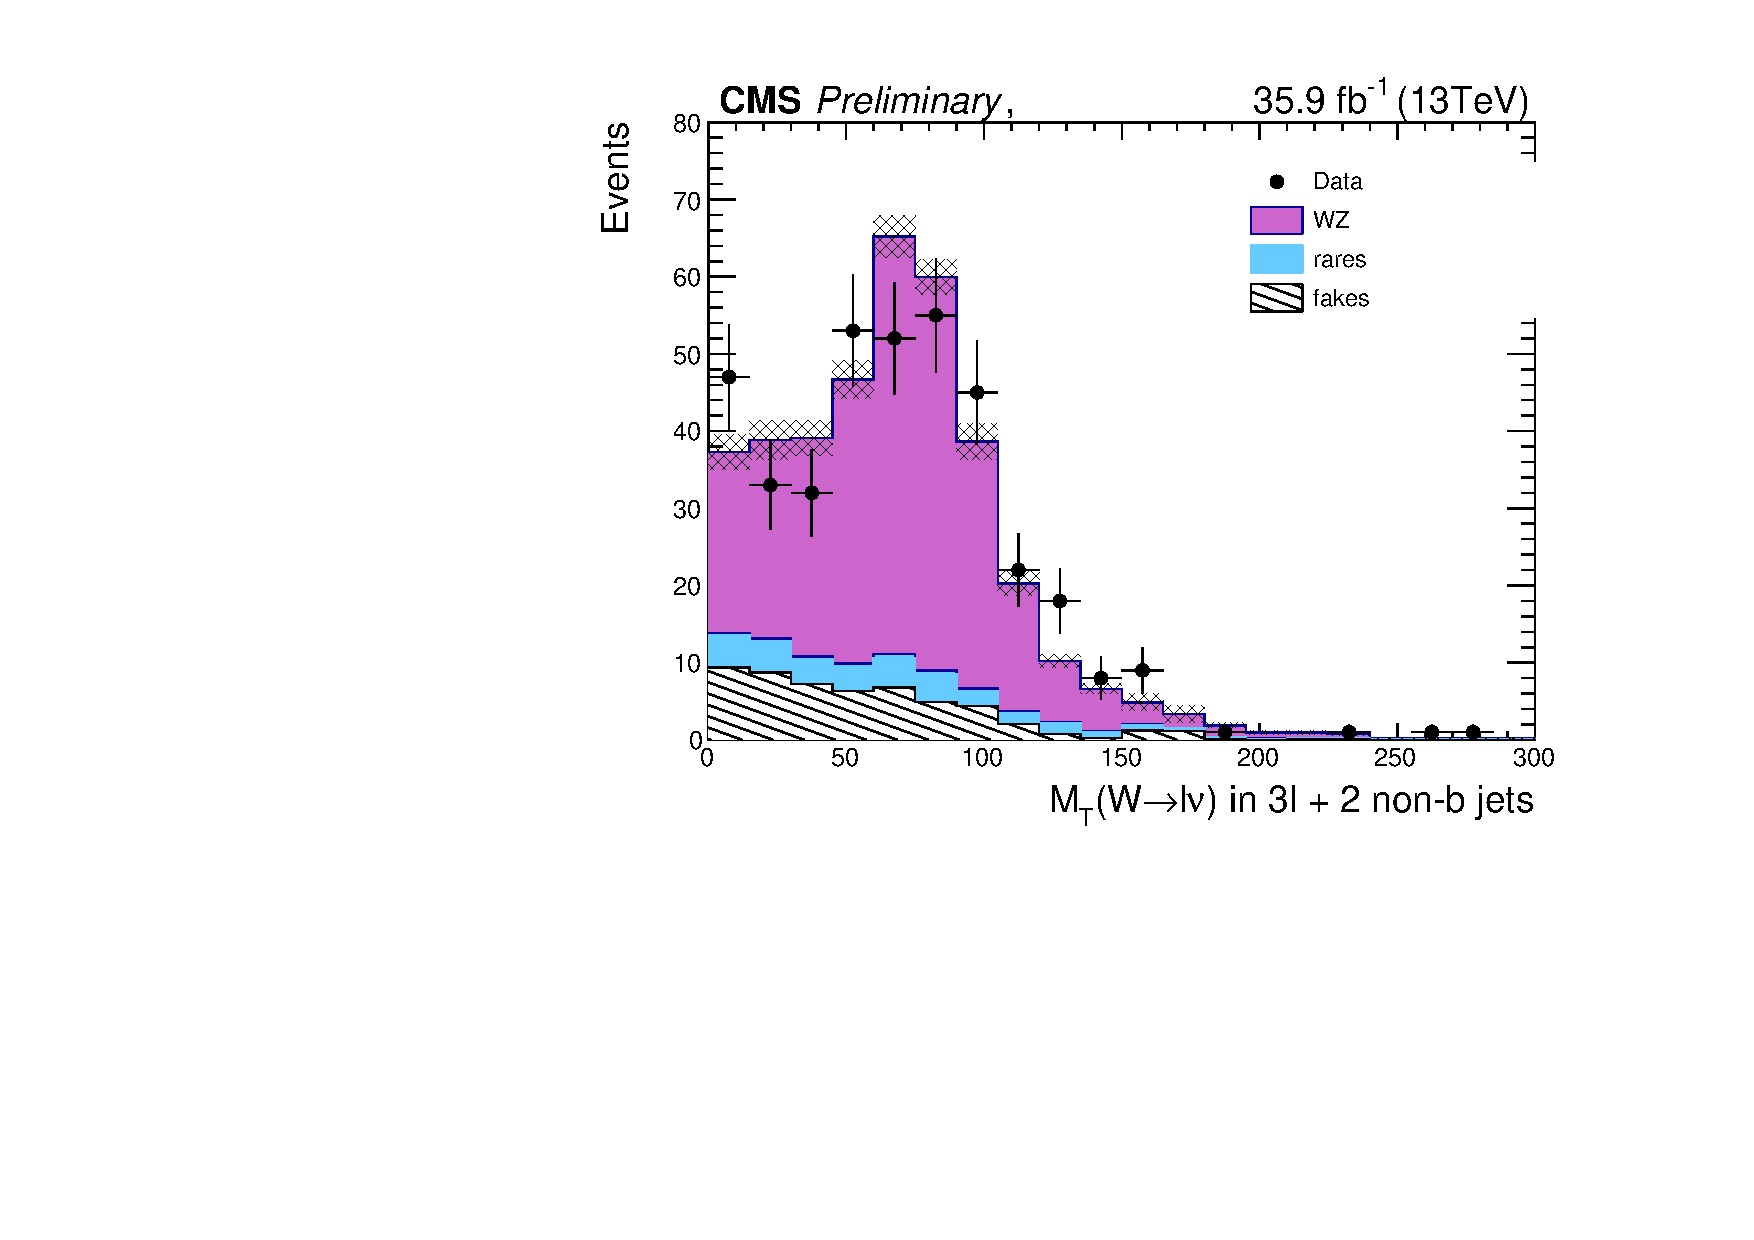
\includegraphics[width=0.48\textwidth]{plots_dibosons/WZ_3l_2nonbjets_MTW.pdf}
	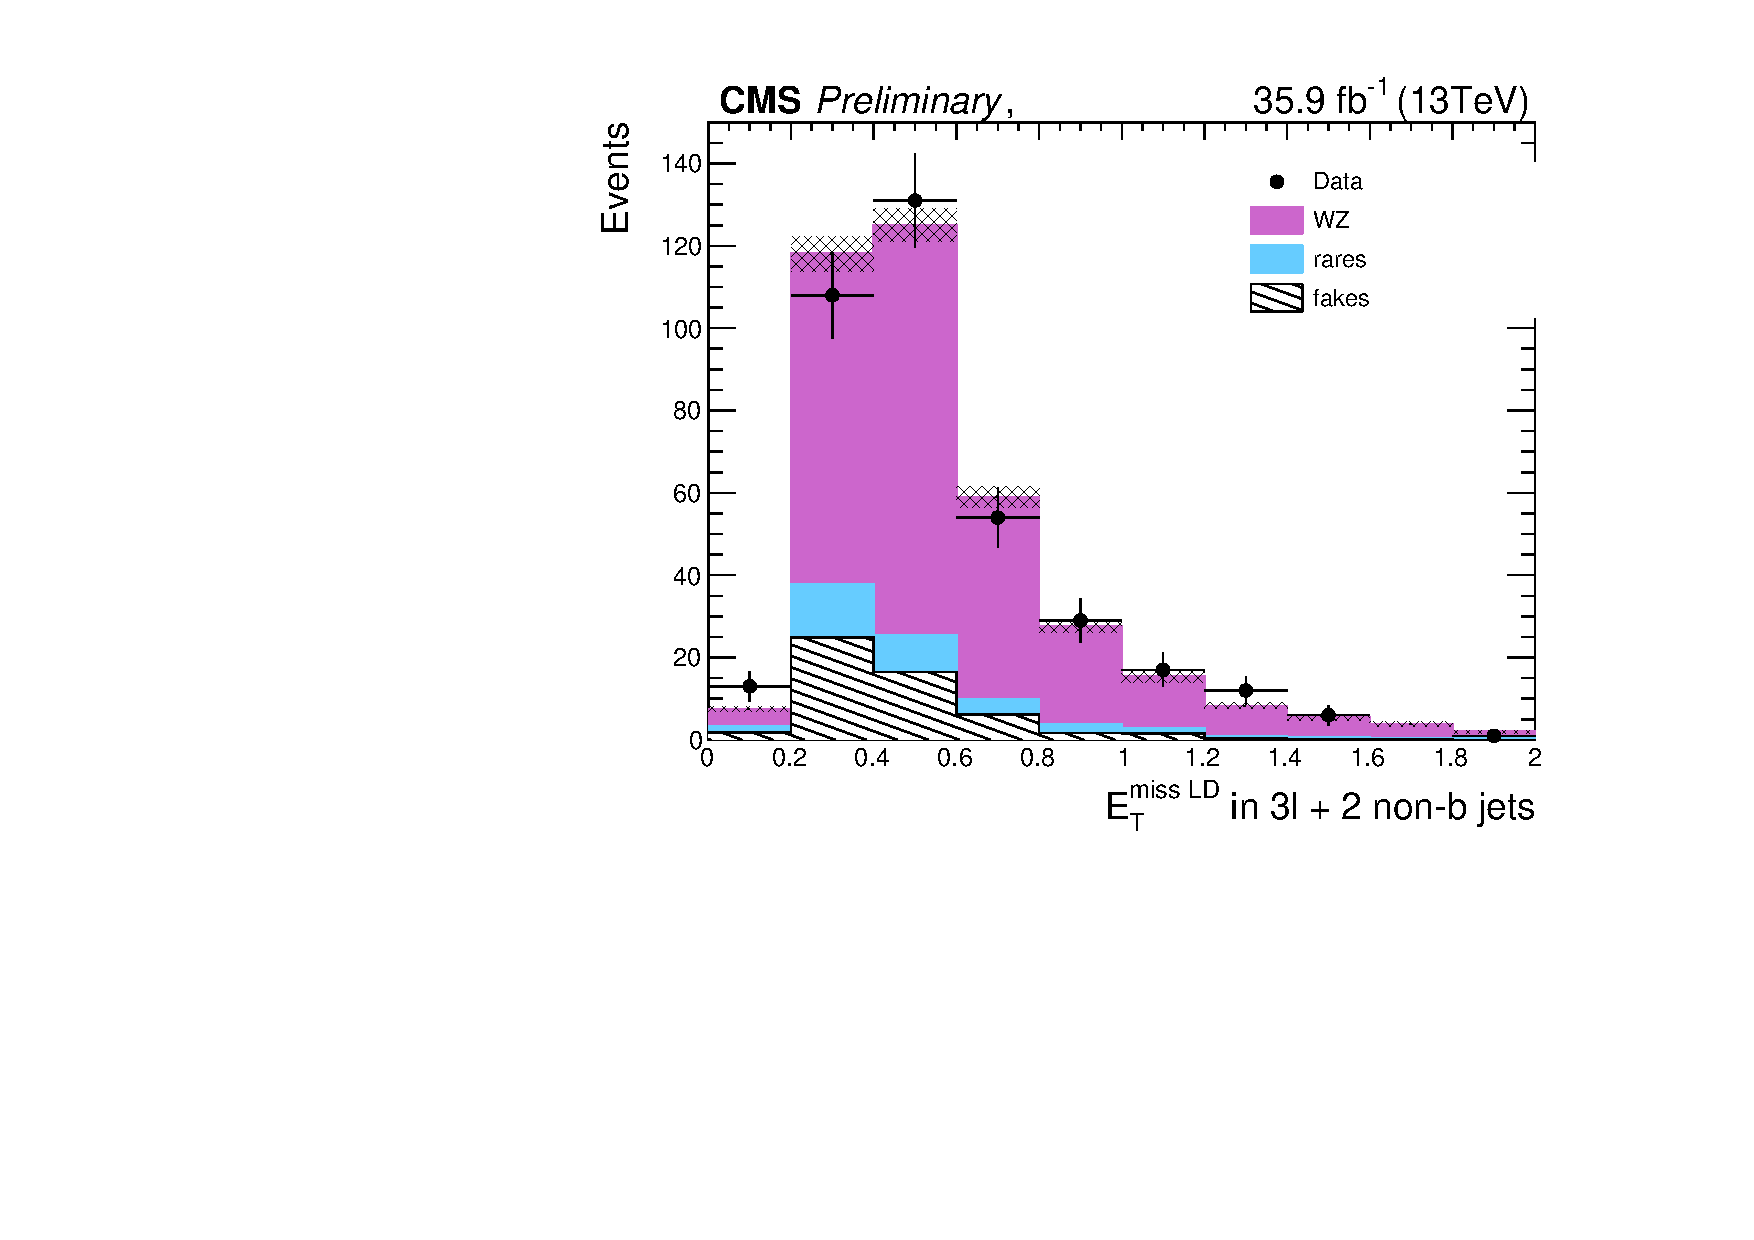
\includegraphics[width=0.48\textwidth]{plots_dibosons/WZ_3l_METLD.pdf}
	\caption{
	Distribution of the transverse mass of the lepton not associated to the reconstructed Z boson, $m_{T}(l)$, (left) and transverse missing energy, $met$, (right) after a fit of the WZ and beckground processes to the data.
	}
	\label{fig:RescalingWZ}
\end{figure}

\subsubsection{Extrapolation to events with b-jets}

The ratio of the events yields between signal region and control region is measured in the simulation.
The main systematics are expected to come from the b-tagging scale factors since most of the WZ plus two b-jets events are due to mistags:

$$\text{SR-b-loose/CR} : 0.0371  \pm  0.0041 \text{ (b-tagging) }  \pm  0.0028   \text{ (theory)}$$
$$\text{SR-b-tight/CR} : 0.0015  \pm  0.0006 \text{ (b-tagging) }  \pm  0.0001 \text{ (theory)}$$

Theoretical uncertainties arise from the modelling of the heavy flavour content of the jets in diboson plus multijet events. The expected flavour composition for WZ events passing the b-loose (resp. b-tight) jet selection is approximately 35\% (13\%) of events with mistagged jets from gluons or u,d,s quarks, 47\% (50\%) of events wit a jet from a charm quark or antiquark, and the remaining fraction from events with a least one bottom quark or antiquark. Uncertainties on the extrapolation arising from the parton distribution functions are estimated by simulated reweighting of the events to different PDGs sets and all their associated eigenvectors or replicas.

The overall uncertainty on the normalization of the $\PW\Z$ background
is composed by  the statistical uncertainty in the control
region, from the residual backgrounds in the control region, from the uncertainties on the
$\cPqb$-tagging efficiencies, from the parton distribution functions
and from the theoretical uncertainties on the extrapolation
(dominated by the uncertainty on the flavor composition of the final
state due to higher-order QCD terms).

%The overall uncertainty on the normalisation of the WZ background is n\%: n1\% from the statistical uncertainty in the control region, n2\% from the residual backgrounds in the control region, n3\% from the uncertainties on the b-tagging efficiencies, n4\% from the parton distribution functions and n5\% from the theoretical uncertainties on the extrapolation.

%\begin{table}[h]
%\centering
%\caption{Cross sections for WZ production in association with jets containing charm quarks of antiquarks (c) or any flavour of quarks except the bottom (j) for the nominal choice of the renormalization and factorization, for twice that value (scale up) and half of that value (scale down).}
%\label{tab:crosssectionWZ}
%\begin{tabular}{ccccc}
%\hline
%process             & order       & nominal          &  scale up         & scale down     \\
%\hline
%$\sigma(WZ+c+j)$     &             &                  &                   &                \\
%$\sigma(WZ+j+j)$     &             &                  &                   &                \\
%\hline
%$\sigma(WZ+c)$       &             &                  &                   &                \\
%$\sigma(WZ+j)$       &             &                  &                   &                \\
%\hline
%\end{tabular}
%\end{table}







